\documentclass[phd]{abdnthesis}

%% For citations, I would recommend natbib for its                          
%% flexibility, particularly when named citation styles are used, but                
%% it also has useful features for plain and those of that ilk.                      
%% The natbib package gives you the following definitons                             
%% that extend the simple \cite:                                                     
%   \citet{key} ==>>                Jones et al. (1990)                              
%   \citet*{key} ==>>               Jones, Baker, and Smith (1990)                   
%   \citep{key} ==>>                (Jones et al., 1990)                             
%   \citep*{key} ==>>               (Jones, Baker, and Smith, 1990)                  
%   \citep[chap. 2]{key} ==>>       (Jones et al., 1990, chap. 2)                    
%   \citep[e.g.][]{key} ==>>        (e.g. Jones et al., 1990)                        
%   \citep[e.g.][p. 32]{key} ==>>   (e.g. Jones et al., p. 32)                       
%   \citeauthor{key} ==>>           Jones et al.                                     
%   \citeauthor*{key} ==>>          Jones, Baker, and Smith                          
%   \citeyear{key} ==>>             1990                                             

\usepackage[numbers]{natbib}
\usepackage{hyperref}
\usepackage{scrextend}
\usepackage{pdfpages}
\usepackage{float}
\setlength{\bibsep}{0pt}
\bibliographystyle{apalike}

\usepackage[T1]{fontenc}
\usepackage{makecell}

\title{Using Natural Language Processing for Automatic Generation of Animated Dialogue Scenes in Video Games}
\author{Mikolaj \ Panasiuk}
% IMO this is a bit silly, but some like to include these. To remove,
% delete this declaration and remove the option from the
% \documentclass definition above.
%\qualifications{PhD, Computer Science, University College London, 1997\\%            
%BEng (Hons.) Electrical and Electronic Engineering, The University of Wales, Swansea, 1992}
\school{Department of Computing Science}

%%%% In the final submission of a thesis, this should only be the year
%%%% of submission.  However, it is useful to use \date{\today} for drafts so that
%%%% they don't get mixed up.
    
\date{2018}
\newcommand \videoshost{\url{http://mpanasiuk.me/bscthesis/samples.zip}}

%% It is useful to split the document up as chapters and include
%% them.  LaTeX will sort out all the numbering and cross-referencing
%% for you --- if you run it enough times!

%% If you want to include only a couple of chapters then use the
%% \includeonly{} command with a list of the file/chapter names that
%% you wish to include.  NB, this must be in the preamble.

\includeonly{introduction,background,analysis,faq, design, requirements, testingperf, usermanual, maintenance, evaluation, results, otherappend, conclusions, discussion}

\def\sfthing#1#2{\def#1{\mbox{{\small\normalfont\sffamily #2}}}}

\sfthing{\PP}{P}
\sfthing{\FF}{F}

%% This will make sure that all cross-references are correct (including
%% references to those file not included) but will produce a dvi
%% file with only those files/chapters you specify included.

\begin{document}

%%%% Create the title page and standard declaration.

\maketitle
\makedeclaration

%%%% Then the abstract and acknowledgements

\begin{abstract}
  Modern video games (especially those of the RPG genre) can feature over a hundred hours of dialogue. During a dialogue scene the characters are expected to behave naturally and use body language in a way that is `normal' and corresponds to what they are saying. Due to the sheer amount of dialogue animation needed it is impossible to animate all the scenes manually. Many solutions to automatic generation of such scenes (most of which are not available publicly and produce animations that still require a fair amount of manual work) have been tried with mixed results.
  
  This project aimed to develop a tool capable of generating 3D animated dialogue scenes with virtually no manual labour required. This is achieved by using natural language processing to extract the mood of characters directly from script and using a database of pre-recorded motion capture animations to assemble a dialogue scene. Additionally, the tool was aimed to be cross-platform, easy and cost-efficient to use, as such a tool would be most useful for small teams and amateur developers.
  
  The tool was evaluated by a real audience whose task was to compare scenes from actual games with scenes generated by the developed software. The tool succeeded in creating rather convincing animation that was often described as more enjoyable or engaging than the animations from games; Unfortunately the generated scenes lacked realism and the NLP approach was not accurate enough when dealing with sarcasm or ambiguity. Because of those issues the project did not achieve a full success.
  
  The software itself would need some serious improvements before becoming commercially viable. It is however developed enough to prove the usefulness of NLP in game animation. This approach has a potential to be incorporated into a larger animation generation framework (where other approaches besides NLP collaborate to create the most lifelike animations) and even to be extended into other areas of computing science such as robotics. 
\end{abstract}

\begin{acknowledgements}
  First and foremost I would like to thank Professor Ehud Reiter for his invaluable guidance, supervision and patience. 

  Secondly, I would like to thank the Blender Foundation for providing free, open-source, modern 3D content creation tools for over 15 years and the Max Planck Institute for Biological Cybernetics for making the Emotional Body Motion Database available publicly.
  
  I would also like to thank the BioWare Montreal studio for developing \textit{Mass Effect: Andromeda}. The game famously suffered from multiple issues in many areas of game development. Its weird and unnatural dialogue animation constantly broke the player's immersion and turned serious moments into comedic scenes. The following blank-verse poem commemorates the achievements, the failure and the disbandment of the BioWare Montreal studio:
  
{
  \fontsize{9pt}{6pt}\selectfont
	  \bigskip
	  \noindent \textbf{BioWare Montreal}\newline
	  It seems like we hardly knew you,\newline
	  probably because you only existed for nine years and were relatively small\newline
	  The more surprising is the fact that\newline
	  you have been put in charge of the most significant of BioWare's franchises\newline
	  \newline
	  Pity,\newline
	  because you looked like a pretty cool place to work at\newline
	  Even though Glassdoor reviewers complained that there are no windows at the office\newline
	  and that they all feel like nocturnal creatures.\newline
	  Montreal also seems like a good place to live I guess\newline
	  despite all the snow in the winter and the roadwork in the summer\newline
	  But how would I know, I have never been to Canada anyway\newline
	  \newline
	  You should have went gently into that good night\newline
	  But you didn't\newline
	  And now your game is a laughing stock for the entire gaming community\newline
	  Press F to pay respects\newline
	  F
}
  
  
  
\end{acknowledgements}


% Tables 
\tableofcontents
\listoffigures
\listoftables

% Body
\chapter{Introduction\label{chap:introduction}}

Each chapter heading is typeset in this way --- this in an integral
part of the style, so if you don't like it abdnthesis.cls may not be
for you. However, do feel free to modify the .cls file to your needs.

\section{Defaults}

\begin{itemize}
\item oneside --- assuming single sided printing.

\item onecolumn --- \LaTeX\ will give you an error if you try to use
  the twocolumn option, not that anyone would contemplate this for a
  thesis.

\item 11pt --- this works best with the text height and width on A4
  paper.

\item 1.5 line spacing --- looks much better than double spacing.

\item Times Roman font --- for both text and maths with the exception
  of mathcal, but see below for options.
\end{itemize}

\section{Options}

\begin{itemize}

\item These are mutually exclusive options that are used to specify
 the type of degree that the thesis is to be submitted in partial
 fulfilment of the requirements of:

\begin{itemize}
\item phd or PhD -- the default.
\item mphil or MPhil -- for Master of Philosophy Theses.
\item msc or MSc -- for MSc project reports.
\item bsc or BSc -- for BSc project reports.
\end{itemize}

\item Two self-explanatory options for changing the line spacing from
 the default 1.5.

\begin{itemize}
\item singlespace
\item doublespace
\end{itemize}

\item titlebox --- this option ensures that the title of the document
 fits within the window on the standard departmental BSc or MSc
 project report front cover.
 
\item twoside --- this option is if you wish to print your thesis
  using a double sided printer.  Note that the University regulations 
  do not permit the submission of theses printed double sided.

\item cmmath --- this action changes the font used in math mode to be
  Computer Modern. The default is for all math mode fonts to be times
  with the exception of the mathcal font. If you want to also use
  times for mathcal, you need to comment out these two lines in the
  abdnthesis.cls file:
\begin{verbatim}
        \SetMathAlphabet{\mathcal}{normal}{OMS}{cmsy}{m}{n}
        \SetMathAlphabet{\mathcal}{bold}{OMS}{cmsy}{b}{n}
\end{verbatim}

\item cmall --- if you want to go with Computer Modern for both
  text and maths, use this option.
\end{itemize}

There is also an \emph{optional} command for including prior
qualifications within the title page; some like to do this. Prior to
version 2.3 (2013/08/11) \LaTeX\ would give an error if this was not
declared, even if you didn't want this information on the title
page. This meant that you would have to have made the declaration
\verb+\qualifications{}+, which was an ugly solution. Now, ``empty''
declaration can simply be omitted.




\chapter{Background and Related Work \label{chap:background}}

\section{Background}
Manually crafting every animation in the game is unrealistic due to cost and time requirements. Many games have employed various approaches to computer generated animation in order to generate hours of realistic content. No game however has succeded in making the dialogue animation indistinguishable from manually animated cutscenes.

\section{Existing Systems}

There has been a variety of approaches featured in games. Many of them ended up generating dialogue scenes that are higly repetitive, not very realistic and in general not mathing the sentiment and emotion of the speech with movement. The only system that did not seek to find cheap workarounds around the issue and instead embraced the full complexity of the problem is the dialogue sene generator used in The Witcher 3. The system developed by CD Projekt Red made computer generated dialogue sequences in many cases barely distinguishable from those made by an artist, allowing less important scenes to be left completely untouched by a human animator. ~\cite{pcgamerwitcher}


The tool created by CD Projekt Red takes information on initial state of involved characters (position, stance, emotions, etc.) and audio recording of the dialogue lines. The tool chooses matching premade animated clips and outputs a fully editable animated scene of characters conversing with one another. The tool uses audio recordings to aid the animated clips (analyzing the audio waves may help decide when characters accent or underline some information). This tool is the current state-of-the-art and has produced the best effects in terms of amount of work to quality of animation ration. However, there are some serious drawbacks to this project. It still requires a fair amount of work as for every scene the initial state must be specified manually. Moveover, the system requires audio to be recorded first. Moreover, the tool is not released to be used commercially outside CD Projekt. ~\cite{gdcwitcher}


The tool I propose be able to hardly compete with that of CD Projekt Red, however it would have some significant advantages. It would make generating the scenes even faster (requiring less manual work and preparation) and would in general be more appealing to small developers and people who are not animation experts.

\section{Related Work}
The main focus of this project is the usage of NLP for generating animated sequences. While this project puts particular emphasis on generating scenes of dialogue, there exist a multitude of projects that explores the usage of NLP in animation in a variety of ways.

\subsection{Generating Animated Scenes for Training and Instructions}
A very early research (1991) explores usage of NLP for creating animations that would help engineers demonstrate tasks in an easy and safe way (demonstrating tasks personally might be unsafe, reading manuals might be insufficient to understand the task in full)~\cite{animosha}. The system would take as input a set of natural language \textit{directives} or \textit{commands} (e.g. \textit{move cup to table}). The system would interpret such an instruction into a series of steps (tasks) that are carried out in a given order. Based upon that sequence an animation would be generated.

The project hovewer seems to have a few significant problems. Most importantly, the end results was not editable. In my research I believe that the end results will not be immediately satisfactory without any manual improvements and I believe that the outputted scenes should be fully editable. The other issue with this project is that the end result is not realistic or immersive (this was not a priority of that research, but is important for me). The animations were automatically generated in full, which I do not believe to be a viable approach for my project. To improve realism of the scenes, the animation should be created using motion capture clips.

\subsection{Animation From Text and Motion Database Framework}
This research project explores a topic much closer to mine. It does not put any emphasis on emotions or gestures (just actions), however it proposes a usage of motion capture database ~\cite{animmc}.


% ----------------------------------------------- %


\section{Emotion Analysis}

The task of emotion analysis is a subset of natural language processing. The task of analysing natural language text in search of subjective information such as sentiment or emotion is known as sentiment analysis.

\subsection{Sentiment Analysis}
Sentiment Analysis can be broadly defined as a computational approach for discovering opinions and attitudes expressed in text by opinion holders. In its most basic form it focuses on binary classification of the sentiment of the opinion holder (positive or negative) ~\cite{sentimentanal1}, but can be extended to mine for more complicated opinions such as emotions or detecting sarcasm. One of the popular uses of sentiment analysis is predicting stock market behaviour, as well as getting immediate feedback on products, political campaigns, decisions by monitoring social media ~\cite{sentimentanal2}.

Approach to sentiment analysis might differ depending whether focus is on document-level analysis or sentence level analysis - where document-level analysis assumes the entire document to have one clear area of focus, while sentence level analysis analyzes each sentence individually. Apart from those, there are more types of sentiment analysis such as aspect-based analysis (which is use when the document or sentence does not focus on a single entity), or comparative analysis (when direct opinion is not desired, but it is needed to contrast opninions with each other)~\cite{sentimentanal2}. For the purposes of this project, it seems that the sentence-leve approach is the most suitable, as dialogues comprise of mostly single-sentence lines (rarely more than three sentences per line) and emotional payload may change as the dialogue progresses.

Traditionally sentiment analysis is performed by various classification mathods (usually supervised learning). Naive Bayes classifier and support vector machines were proven to yield pretty acurrate results (over 80\% accuracy in general) ~\cite{sentimentanal1}. The major constrait of those methods is that their quality is tightly linked with the quality of the lexicon used and size and quality of training datasets.

One state-of-the-art solution to emotion analysis problem has recently became publicly available. Created by IBM, Watson Tone Analyzer is a tool capable of accurate emotion labeling (fear, joy, anger, etc.) as well as tone labeling (analytical, confident, tantative, etc.). The system is based on the \textit{Big Five personality traits} model ~\cite{watson}.



\section{Animation Software}

The output scene must be created in some software able to play and use the scene. Developing a tool for this would be too time consuming - such software is not a small undertaking and with the time constraints this would result in a very rudimentary framework that would be very limiting. Therefore a choice must be made between existing frameworks.

The animation software must satisfy the following requirements:
\begin{itemize}
\item Flexibility and editability - As the scenes created by the generator will not be perfect, the software must provide powerful animation editing features.
\item Exporting - It is desirable for the animation to be able to be exported into variety of different formats that can be used by other frameworks useful within game development.
\item Availability - As the proposed tool is developed with small developers in mind, it is most desirable for the tool to be available without any unnecessary fees or licensing. The proposed tool shoul also provide help for people unfamiliar with animating, who would be unwilling to pay additional fees for something they are not familiar with.
\item Familiarity - Although most animation software is based on similar concepts, due to time constraints my previous experience with the software is also important.
\end{itemize}


\subsection{Maya}
Maya is a 3D computer animation software developed by Autodesk. It supports modeling, rendering, simulation, texturing, and animation. This software is an industry standard and has been used for such projects as the Halo franchise. It supports all the animation editing and exporting features needed for this project, however it comes with a pretty harsh pricetag of \$180 per month \footnote{\url{https://www.autodesk.com/products/maya/subscribe}}; a price which would make the potential reach of the proposed tool much smaller. Moreover, although I am familiar with animation concepts, I am not familiar with Maya.


\subsection{Blender}
Blender is an open source animation software. Similarly to Maya, it supports modeling, rendering, simulation, texturing and animation. Due to its open source nature the software may be less usable or stable at times however it is still very powerful and recognized within the industry. Blender's rendering engines are not as sophisticated as those of Maya. It supports exporting the animations to Collada, Alembic, 3D Studio, FBX, Motion Capture (.bvh), Wavefront, X3D and Stl file formats. This means that the final animation could be exported and used by pretty much any other tool. Blender is completely free to use and available to anyone. I am familiar with the tool


\subsection{Unreal Engine}

Unreal Engine is by far the most popular and most powerful publicly accessible game engine. Since the proposed tool would find most use in games it would make sense to create the scenes directly in a game engine. This approach however has some disadvantages - animation editing features in game engines are much more limited than those of a software dedicated to creating animation. Moreover, any game engine will not support the same exporting features (however, since the animation would already be in the engine, the need for exporting is arguable). Unreal engine is free to use, however Epic Games will seize a portion of income generated by a product developed with Unreal Engine. \footnote{\url{https://www.unrealengine.com/en-US/faq}}

\subsection{Unity 3D}

Unity 3D is the most popular freely available engine after Unreal. It suffers from the same drawbacks regarding animation editing features and is in general less stable and sophisticated. The only reason why Unity would be more suitable than Unreal for this project is my familiarity with the Unity 3D framework.


\subsection{Final Choice}

Upon taking a closer look on the available software, I conclude that Blender is the most suitable tool for the task as it satisfies the requirements best. It provides all the necessary editing exporting and editing features, is free and easily available and I already have experience with using it.







\chapter{Analysis \label{chap:analysis}}

\noindent The project  methodology,  development  tools  and  technologies  and  project  risk assessment are defined in this following chapter.


\section{Methodology}

The activities required in order to develop the project are listed below:

\begin{itemize}
\item Develop a project plan.
\item Review literature. Review existing software, learn about other approaches, analyze existing research.
\item Find and assemble a set of relevant motion capture animated clips.
\item Prototype a module that uses processes the script and outputs a structured file that can be used to generate the animated scene.
\item Tag and classify animation clips. Categorize clips by emotion, length, etc.
\item Prototype a Blender extension that uses the created structured files to output an animated scene.
\item Iterate on the existing software adding new features.
\item Evaluate the prototype with real audience.
\end{itemize}

The generated animation must be evaluated with help of a real audience. How animation is perceived is subjective and cannot be decided by one person only. The evaluators will be asked to watch animated dialogue clips from various games and then watch this dialogue recreated using the proposed software. The evaluators will be asked to fill an evaluation survey. This way it will be possible to determined the usefulness and succesfulness of the proposed software.


\section{Technologies and Resources}

\begin{enumerate}
\item Emotion analysis - The first module of the project focuses on NLP. This module should be extract emotions and actions from the script. The most important tool used will be IBM Watson Tone Analyzer. If that tool turns out to be for any reason ineffective or imperfect, a customary tool (naive bayes classifier or a keyword classifier) can be built for that task. Actions can be extracted using a variety of information extraction software such as MITIE or Ollie.

\item Motion capture - The EMBD (emotional body motion database) will be used to source the animations of body movement and gestures. The database provides the recordings as BVH files which is convenient as most animation software (such as Blender or Maya) can import BVH files. The emotional metadata about the animated clips will be stored in an SQLite database. Storing the data using this method will allow the data to be easily and quickly searchable while less complicated than using a full fledged database software (such as MySQL od PostgreSQL) (very few tables are needed, there is no need to use advanced DB software).

\item Animation software - As aforementioned in section ~\ref{sec:animchoice}, the animation software that satisfies all the specified requirements is Blender. Blender supports all the necessary modelling and animation features. It also supports creating extensions allowing the animation to be created and assembled by code.

\item Programming - Python 3 will be used to implement the software. Python is the only language supported for add-on development for Blender. For other modules that do not rely on Blender, Python was chosen due to its development speed and in order to keep consistency among modules.

\end{enumerate}

\section{Risk Analysis}
\label{sec:riskanal}

\begin{table}[!ht]
	\centering
	\small
	
	\begin{tabular}{ |p{11em} |p{23.8em}|p{4em}| }
	 \hline
		\thead{Risk} & \thead{Mitigation} & \thead{Level} \\
	 \hline
	 	Time delays caused by workload/illness & Follow the project plan closely. Focus on developing a minimum working prototype first. & High \\
	 \hline
		Natural Language Approaches are too inaccurate & Use more structured software. Try to find other approaches to this problem. If there seems to be no solution, I can use the findings and existing software to argue that the technology has not yet reached a level that would make this project viable.  &  Low \\
	\hline
		Motions obtained from the EBMD are not expressive and unambiguous enough to create realistic and convincing scenes & Even with bad quality animations it should be possible to determine whether this project has future potential, given a better motion capture database is used. & Moderate \\
	\hline
	\end{tabular}

	 \caption{Risk Assessment}
	 \label{tab:riskassessment}
	 
\end{table}
\chapter{Requirements Specification\label{chap:requirements}}

\noindent This section describes functional and non-functional requirements of the proposed software.


\section{Functional Requirements}

\noindent {\bf FR1 Analysis of a semi structure script}

\noindent The software takes a semi structured script as input. The structure of a script must resemble a structure of a movie script. The script provides 3 kinds of information - characters involved in a scene, dialogue lines and actions performed by characters during the scenes. The software must be able to extract actions and emotions from the script.

\bigskip

\noindent {\bf FR2 Find relevant animation clip}

\noindent The software must take information about character's emotions and actions and choose animation clip that best represent's characters behaviour.

\bigskip

\noindent {\bf FR3 Assemble final scene}

\noindent The software takes information generated by other modules and outputs an animated scene. The outputted scene must be fully editable, enabling various adjustments before rendering.


\section{Non-Functional Requirements}

\begin{itemize}
\item The user should be able to use the software with a custom motion-capture database (Usability).
\item The user should be able to assign differenct character models to different characters (Usability).
\item The user should be able to fully customize and edit the final scene (Usability).
\item The software is designed to automatically create big amounts of animated scenes. The time of generating a scene is not a high priority, but it must be reasonable (Peformance).
\item The software must support common animation file formats (fbx, bvh) (Portability).
\end{itemize}

\chapter{Design\label{chap:design}}


\chapter{Testing and Performance \label{chap:testingperf}}

This section describes the testing and the potential issues of the developed software.

\section{Components}
The testing of the components was an ongoing activity during the development process - the creation of the software alternated between phases of development and testing. The components were fed typical and erroneous inputs and their outputs were verified for correctness. The testing phase continued until all discovered issues were taken care of and the development could continue.

\section{Analyzer}
There are a few issues that the user should focus on before providing input to the first module. Firstly, the input must be in English, as the emotion analysis is set to only use the English language. The user should make sure that the text they intend to analyse is in English and does not contain non-English characters.

Secondly, the user must make sure that the character names and their dialogue lines are correctly indented. The module was designed to be able to analyse scripts copied directly from the Internet Movie Script Database. Those scripts often have other information (non-relevant to this software) specified at different indentation levels. The software simply ignores that information - therefore, if any of the important information is specified at a wrong indentation level, it will be ignored.

\section{Matcher}
The testing of the matcher aimed to make sure that the matcher outputs animations of correct emotional sentiment and length. There is no other way to do that than to test it empirically. The module was fed with emotional values and text lengths. Whether the output animation matched the emotions provided and its length felt natural (just enough time to read the subtitles, as one would while watching a film) was assessed manually. The module (along with the database) was fine-tuned until it gave satisfying results.

\section{Animation Generator}
There are some serious limitations to the testing of this module. It is hard for a computer to decide whether the animation looks natural. Some animations imported from EBMD experience import problems which results in an animation with broken and unnatural movements. While manually analysing the emotional values of the animations, it was important to check each animation for movements that may have been incorrectly imported. Such animations could not be used with the software and had to be removed.

The animation generator is able to handle only up to two characters in the scene (although the module was designed with extensibility in mind). If a scene JSON file contains information on more than two characters (or no characters at all) the scene will not be assembled and an error message will be displayed instead. In case the scene file is corrupted and cannot be parsed the user will also be presented with an error message. The JSON file can become corrupted if a user does manual changes to it or if the input of the script analysis module is in a wrong format.

\section{Scalability}
The system was tested with inputs of at least fifty lines of dialogue. The system was able to generate the scenes successfully and in reasonable time (more on time of execution in section ~\ref{sec:perf}). A user would rarely need to generate a single scene so long and would rather produce a multitude of shorter ones. However, this shows that the software is perfectly capable of scaling up by allowing the user to create long dialogue scenes.

\section{Samples}
Sample inputs and outputs of the system can be accessed using this link: \videoshost

\section{Performance \label{sec:perf}}
One of the important requirements of the software was the speed of execution. Analysing a dialogue consisting of 6 lines (an average dialogue length used while testing the software) using the first module takes up to 18 seconds. The matcher module is so quick that it's execution does not influence the total execution time (it's execution time could increase provided a bigger animation database). The generator module takes another four seconds on average. This results in an execution speed of about 3.6 seconds per dialogue line. This fulfils the requirements as the time required to assemble an animation is incomparably less than doing it manually and is not a limitation for an animator working on the scene.
\chapter{Evaluation \label{chap:eval}}
This chapter describes how the system was evaluated and explains why such a method of evaluation was chosen. The evaluation aims to determine whether the created system was successful or not and due to what reasons. 

\section{Problems with evaluation}
Evaluation of animation is quite problematic in nature. The main issue is, that how an animation is perceived is very subjective - it is near impossible to computationally determine whether an animation looks natural, whether an animation goes in pair with the speech and if the whole `feel` of the dialogue scene is good. It is then important for the animation to be judged by people. I myself however am not fit to do that - I have spent far too much time creating the animated scenes and watching both failed and successful results. Because of that I am obviously seriously biased and cannot judge the animations from an objective standpoint.


\section{Survey}
In order to account for my bias, I have decided to use interview people about the generated animations. People who have not had a part in the development of the software can provide valuable opinions.


\subsection{Methodology}
People may find it hard to provide an opinion about the quality of an animation if they have nothing to base their answer upon (especially if they are not animators or developers). There needs to be some sort of a benchmark, or a control sample to enable people to judge the animations more efficiently.

To account for that I have chosen the following approach: I would first find a dialogue scene in a relatively popular, successful game and recreate it using the developed software. The participants would be shown both the original and recreated scene and describe how they compare - they would be asked to decide whether using the software has improved or decreased the quality of the scene. 

\medskip
\subsubsection{Preparation}
I have chosen three games from which I extracted the dialogue scenes. I did not want to extract a few dialogue scenes from one game in order to provide variety, but I also did not want to use more than three games as this would make the questionnaire too long and make the participants loose interest or become confused.

The three games are all of the RPG genre and differ by their year of release - I have used a relatively old game, relatively new game and a state-of-the-art game - for if the software is deemed to produce animation of lower quality than the state-of-the-art game, comparing it to an old game may help decide whether the software simply needs improvements, or if the approach itself is wrong.

Not simply any game could have been chosen. In my project I have to rely on EBMD to generate the animations - and the motion capture data provided by the database is not suitable for any game. For example, if a game features a lot of soldier to soldier military interactions, it is expected that the characters will behave in a more serious, less expressive manner (I evaluate on that in section ~\ref{sec:otherfindings}). The EBMD does not supply animations that would be useful such a situation and using a wrong game would cause unnecessary confusion of the participants. The chosen games must feature relatively relaxed, natural conversations. This certainly tightens the pool of games and scenes usable for the evaluation, but I believe that the chosen games are a rather representative sample of the RPG genre.

The chosen games are:
\begin{itemize}
	\item Fallout 3 (released in 2008)
	\item Fallout 4 (released in 2015)
	\item Horizon: Zero Dawn (released in 2017)
\end{itemize}

The dialogues from the games were chosen randomly, however there were some constraints that limited the choice:
\begin{itemize}
	\item The scene cannot feature more than two characters (The software was designed with extendibility in mind, however at the moment it does not support more than two characters).
	\item The dialogue has to convey some emotions (dialogues which feature strictly neutral emotions are not truly representative of the software).
	\item The dialogue cannot be exposition dialogue (Why that is the case and what exactly is \textit{exposition dialogue} I explain in sections ~\ref{sec:evalotherfindings} and ~\ref{sec:otherfindings}).
\end{itemize}



Before conducting an interview it is important to know whether the interviewee has experience with games and animations and development. The answers of people knowledgeable in this area might differ from those provided by people new to this area and it might be helpful to be able to distinguish between them.

\medskip
\subsubsection{The questionnaire}
The questionnaire consists of four sections. The first section provides some details about what the software is trying to achieve and what is expected of the participant. This section also asks whether the participant considers themselves to be knowledgeable about games or animations.

The other sections all ask the same set of questions about different pairs of videos\footnote{The animations and videos can be accessed at \videoshost. A sample dialogue transcript with still images of the scene can be found in appendix section ~\ref{sec:samplescene}.}. At the start of each section, the participant will be shown two videos - an original and a recreated dialogue scenes. After watching both of them they will be asked a couple of questions that determines whether they find the videos realistic, whether the animations correspond to the conveyed gestures and whether they think that using the software improves the scenes. The participants are able to evaluate in more detail on the answers if they wish to do so. The questions that are designed to be answered on a linear scale that resembles the Likert scale\footnote{The Likert scale is a psychometric scale created by a psychologist Rensis Likert. It is commonly used in questionnaires in order to determine whether the participants agree or disagree with given statements.}.

The original dialogue scenes were modified in two ways. Firstly, apart from the in-game subtitles, another set of subtitles was added for accessibility purposes. The added subtitles were the same as the original subtitles, but bigger and easier to read. Secondly, the videos were muted. Audio is completely irrelevant to this project. I could not procure audio for the recreated scenes\footnote{Simply overlaying the audio from the original scene over the recreated scene is not a good solution either. The audio was not created with the recreated scene in mind and the recreated scene did not take audio into account. Because of that, the characters would perform body motion that puts stress on one part of a sentence while audio would put stress on a different part of a sentence. This makes the audio unusable with a scene as it would make the scene feel completely unrealistic.} therefore the recreated scenes are mute. People watching first a scene with audio and then a scene without audio would focus too much on that difference instead on the difference in animation. Therefore, it is best to remove any sound from all the videos.

The surveys were conducted as a one-on-one interview if possible. If the participants were unavailable or preferred not to do this personally, an online version of the questionnaire was provided. The participation in the questionnaire was fully voluntary. The participants were presented with a consent form before answering the questions and were provided with the details of the software and how the study is going to be conducted. No aspect of the software or the study was hidden from the participants and they were able to both request more details or quit any time they wished.

As mentioned before, the preferred approach was a supervised survey as it is important that the participants correctly understand what the project is about and what it is trying to achieve. The survey was targeted mostly at my colleagues (Bachelor computing science students), as certain level of computing science and application development expertise is desirable. That is because people who are unacquainted with prototyping and development might focus too much on how unpolished the animation is (since it is only a prototype and the animations are rather crude - there is no background in the scene, no audio and no texturing/graphics) than on the gestures and dialogue itself.

The full questionnaire can be found in the appendices in section ~\ref{sec:appquestionnaire}.

\medskip
\subsubsection{Objectives}
The survey has the following objectives:

\begin{addmargin}[2em]{2em}
	\noindent \textit{To test whether using the NLP approach for animation generation has created scenes that are more realistic and natural than the original scenes.}
	
	\medskip
	
	\noindent \textit{To test whether the animations generated using the NLP method are preferable to those created by traditional methods.}
	\medskip
	
	\noindent \textit{Determine how much manual adjustment is required before the animations generated by the software are satisfactory.}
\end{addmargin}



\section{Other findings \label{sec:evalotherfindings}}
Apart from the findings of the questionnaire, I also wish to describe my own realisations that I devised during the development of the software. I know that I cannot use them to decide the successfulness of the software because of my bias towards it, however, I think that there are a few aspects worth mentioning that will not be discovered by the questionnaire participants.

As I was testing the software many times and I tried to recreate many scenes from RPG games I have noticed that the software does not perform well if certain conditions are not satisfied. For example: the general `feel' of the game must match the gestures provided by the motion database, the software does not perform well with scenes that contain exposition or sarcasm. I will explain those issues in more detail in section ~\ref{sec:otherfindings}.





\chapter{Results \label{chap:results}}

\section{Survey}
The survey was completed by 12 people in total. Half of the participants have described themselves as well-acquainted with the area of games or animation. One person was not sure and the rest was not acquainted with that topic. However it appears that this is never strongly correlated (using Pearson correlation coefficient) to any of the other answers. It seems that having experience in games or animation does not significantly influence how the participants perceived the animations.

The participants were asked to decide whether the animations presented to them were realistic. The question was asked about each of the six scenes. The t-test was performed taking into account the answers about all the original scenes and the recreated scenes. The p-value of 0.7614 shows weak statistical significance of the result. The realism of the scenes was described on a one to five scale\footnote{The participants were asked to say whether they agree with the statement  `video X is realistic'. The answer was taken on a one to five scale where one means `strongly agree' and five means `strongly disagree'}, where the average score for both original and recreated scenes is about 3.1. These results show that animations generated by this project are no more realistic than the originals and that both original and recreated scenes are hardly realistic at all.
	
A similar set of questions was asked about the effectiveness in conveying emotions. The participants were asked to decide whether the animations correctly convey the feelings and emotions of the characters in the scene. This time the results yielded the p-value of 0.4657 showing a higher significance of the result. The participants' answers suggest that the animations reproduced by the software are slightly better at conveying feelings and emotions (the mean score of the recreated animations was by 0.3 (out of 5) better than the originals). These results show a very slight advantage of the recreated animations over the original ones.


\begin{figure}[H]
	\centerline{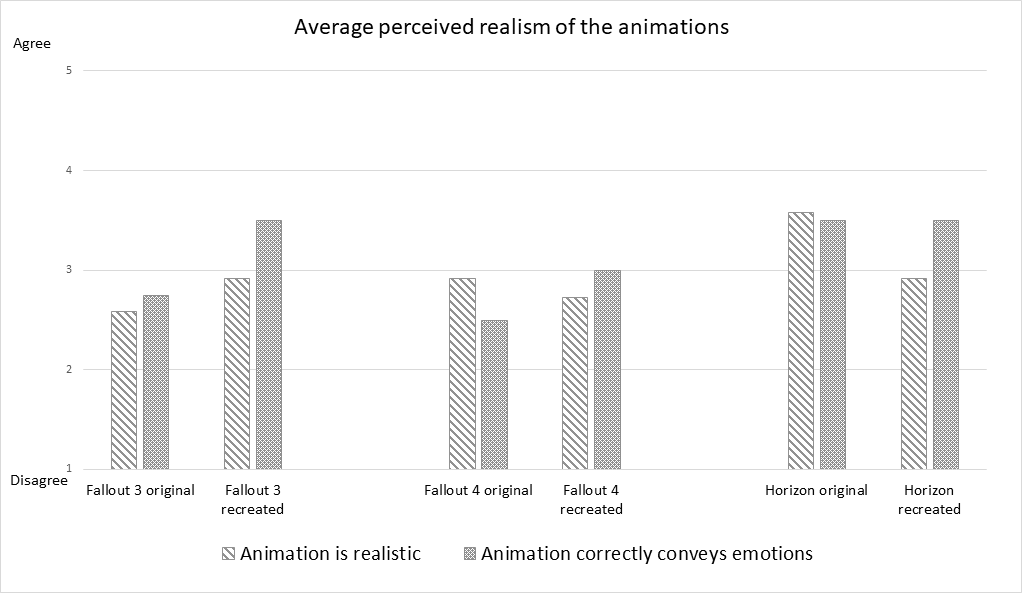
\includegraphics[width = 25em]{img/results/realism.png}}
	\caption{The addon UI}\label{fig:realism_graph}
\end{figure}













\chapter{Discussion \label{chap:discussion}}
This section discusses and evaluates the findings accumulated during the development and evaluation of the software.

\section{Survey results}

\subsection{Realism}
According to the results of the survey the realism of the generated animations is rather disappointing. The animations managed however to be relatively as realistic as an animation from a quite recent game, meaning they might be good enough to be used in a game (given how little it takes to generate them). The very important aspect is that the generated animation were not seen as realistic, but were seen as correct (matching speech with emotions and body language). It is interesting that people often preferred the recreated scenes even when they were less realistic than the originals. Interviewees dissatisfied with the recreated animations said that the movements of characters are `weird' and that the software is too sensitive, with characters overreacting to the actual situation. 

The survey successfully carried out its first objective, showing that the NLP approach did not produce animations more (or much less) realistic than the originals. There are a few explanations to that. The possible causes have been described in section ~\ref{sec:riskanal}.

The lack of realism was probably not caused by the emotion analysis. The interviewees rather agreed that the emotions in the speech match the body language. The results suggest that the problems lies within the movements itself. 

Both the motion capture data quality and the uncanny valley principle are possible causes of those results. It is impossible to say now which one is more important. A similar study which uses a different motion database could be helpful in determining that.

It is also possible that the results are skewed because of the crudeness of the entire scene. The models are rather bulky and poorly detailed, untextured, there is no background or audio. That is because the software focuses solely on the animation. However, the interviewees are not used to watching animation being developed and might instinctively see such a scene as less realistic and be unable to look at the animation fully objectively. Given enough time and resources these issues could be addressed by adding detail to the scene by professional artists and the system should be then evaluated by a truly random audience (not dominated by CS students, with a greater amount of participants).

The generated scenes reach an acceptable level of realism, however they are not realistic enough to deem the NLP method of generating animation to be better than other, traditional ones. 

\subsection{Preference}
Surprisingly, although the generated animations were not highly realistic, they were often preferred to the original ones. It seems that the recreated animation may have been over the top, while in the original scenes there was simply not much going on (the gestures being very subtle and ambiguous). It seems that the participants found the slightly overdone body language more enjoyable and less boring than the blandness and genericness of the originals.

Realism itself is often not a key aspect to a game's success. It might be a great advantage for a game to feature scenes that are similarly or slightly less realistic than the norm when those animations are more engaging. This might be particularly true when a given game is not trying to be realistic (it might be over the top and cartoony on purpose).


\subsection{Adjustments}
The results regarding adjustments of the animation were not surprising. The software was never intended to produce perfect animation which needs no adjustments before shipping (there is hardly any software capable of that). Moderate adjustments of the animation are perfectly acceptable. If this software was ever to become fully commercially viable, it would be a good idea to further develop the animation generation. Better camera work, smooth blending of the movements, etc. can be done automatically and would further minimize the need for manual adjustments.


\section{Other findings \label{sec:otherfindings}}
In previous sections I mentioned that the scenes chosen for the questionnaire are not \textit{fully} representative of all the dialogue scenes in a game. When a scene satisfies some conditions, the software clearly under-performs. Below are some of such cases that I discovered.

\subsection{Mismatch between animation database and the `feel' of the game}
The software produces undesirable results when there is a clear mismatch between the provided gestures and the `feel' of the game. By `feel' I mean the general topic and overtone of the game. For instance, a game such as any in the Mass Effect series has a very strict and militaristic feel. While characters still converse in a more casual environment, a certain level of professionalism is always required of them. A game such as `Yooka-Laylee' also contains a fair number of dialogue scenes, but the general feel of the game is childish and cartoon-like. The conversations happen in a much more quirky and exaggerated way.

I was not able to use the EBMD with the Mass Effect games. The EBMD provides very casual, relaxed gestures when almost every character in the Mass Effect game is military. While without context the scenes looked good, when keeping in mind that the scene happens in a militaristic environment one can immediately see that while the characters move and gesticulate in a natural manner, this is not appropriate in a current situation.

This however is not an inherent problem with the software, as it allows for using a custom animation database. It could potentially be even extended to support a different set of animations for each important character in order to underline their personality even more. However, because I used only EBMD for this project, I am unable to test how successful would the software be with scenes that have different contexts.

\subsection{Exposition dialogue}
In media such as books, films and games exposition is pretty common. Exposition is an aspect of narration that focuses on introducing character's backstories, prior plot events, context and other background information. Because typically games feature less narration than books or films, most of the exposition is handled through the dialogue.

The exposition dialogue is already often unnatural and seems out of place. The software generating those scenes made them seem even less natural. During exposition dialogue, the characters should remain rather neutral, as often they will be describing events that happened in the past, or that they have no direct connection with. The software however will find emotions in such dialogue and make characters overjoyed or fearing while there is nothing happening that would provoke those emotions. In many such dialogue scenes the software was simply over-sensitive.

This problem could potentially be solved if the exposition dialogue was tagged in the script by the writers. The emotions extracted from the text could be decreased by some factor to make them less intense. This of course assumes an increase in manual work required as the exposition dialogue would have to be manually tagged.


\subsection{Sarcasm and ambiguity}
NLP has struggled with sarcasm for a long time. IBM Watson Tone Analyzer seems to be no closer to solving this problem. The dialogues that contain sarcasm are simply misinterpreted and the final scenes look terribly out of place. For instance, a character saying `Oh, I'm so scared!' can be either scared, or indifferent and boasting about their courage. This might depend on the context and the tone of their voice. The software will however always associate this with fear and the resulting scene might use animations that convey opposite emotions to those that were meant to be conveyed.

By looking at many dialogue scenes, it became apparent that there is no way to overcome this problem using NLP only, as there are simply too many variables outside of the text that define possibility of sarcasm (context, setting, personality of the character, recent interactions between characters involved in the scene, shared history between conversing characters). The tone of voice might provide more information that would help solve this problem.

Similarly to the exposition problem, the sarcasm problem can also be solved by tagging it in the script. When using sarcasm the writers could indicate that and provide the intended emotion. That assumes a slight increase in the amount of work required and that all sarcasm present in the script is recognized and tagged.


\section{Summary}
The following is a breakdown of what the software managed and failed to achieve.

\noindent Successes:
\begin{itemize}
	\item The software is able to generate scenes quickly with minimal amount of manual work required.
	\item The animations do not need extensive manual polish before being used in a game (The software needs to provide smoother movements and blending between gestures).
	\item The software is flexible and capable of using custom character models and animation data.
	\item The software is cross-platform and the animations can be exported to a multitude of file formats.
	\item The generated scenes are often more enjoyable than the actual scenes in games.
\end{itemize}

\noindent Failures:
\begin{itemize}
	\item Generated scenes are not any more realistic than those featured in modern games.
	\item The software under-performs when dealing with sarcasm, exposition or ambiguity.
\end{itemize}

\noindent Other key points:
\begin{itemize}
	\item The lack of realism may be caused by the data provided by EBMD.
	\item The animation generation process can be improved further using methods already known to the industry.
	\item The NLP approach might in the future be combined with other methods (such as emotion analysis of the audio) to produce even better results.
\end{itemize}





\chapter{Conclusions \label{chap:conclusion}}
conclhere

% Bib
\bibliography{mybib}

% Appendix
\appendix
\chapter{User Manual \label{chap:usermanual}}
The system is designed to be cross platform, however it is advised to use Windows as it is the only system on which the project was thoroughly tested.

\section{Requirements and installation \label{sec:requirements}}
Before using the software, several requirements must be fulfilled.

\subsection{Software and Libraries}
\subsubsection{Required software}
\begin{itemize}
	\item Python 2.7
	\item Pip
	\item Blender version 2.79 or newer
\end{itemize}

\subsubsection{Libraries}
Only for Linux systems: Download and install library python-dev (or python-devel)

Following python libraries must be installed:
\begin{itemize}
	\item setuptools
	\item watson-developer-cloud
	\item wget
\end{itemize}
\noindent The packages can be installed in bulk by running:

\indent `path\_to\_python/Scripts/pip install -r requirements`

\noindent in the main directory. As Blender usually comes with its own Python environment, you will need to run the command:

\indent `path\_to\_blender/version/python/Scripts/pip install -r requirements`

\noindent To install the libraries for Blender.

\subsection{Install Generator as Blender Addon \label{sec:installaddon}}
The following steps are optional. Installing the module as addon will enable the module to be permanently incorporated into Blender.

\noindent To install the addon:
\begin{itemize}
	\item Open Blender
	\item Open user settings (File > User preferences)
	\item Open Add-ons tab
	\item On the bottom panel press `install add-on from file`
	\item Navigate to `project folder > generator` and double click on `addon.py`
	\item In the search box on the top right corner type `NLPanim` - a greyed-out item called `Object: NLPAnim` should appear
	\item Check the box next to the item
	\item Press `Save user settings` in the bottom left corner
	\item Exit user preferences
\end{itemize}

\noindent The module is now installed as an add-on. In the 3D-view (default view) on the bottom of the right-hand side menu there should appear a tab called `Generate NLP anim` (figure ~\ref{fig:installedaddon}).
	
\begin{figure}[!ht]
	\centerline{\fbox{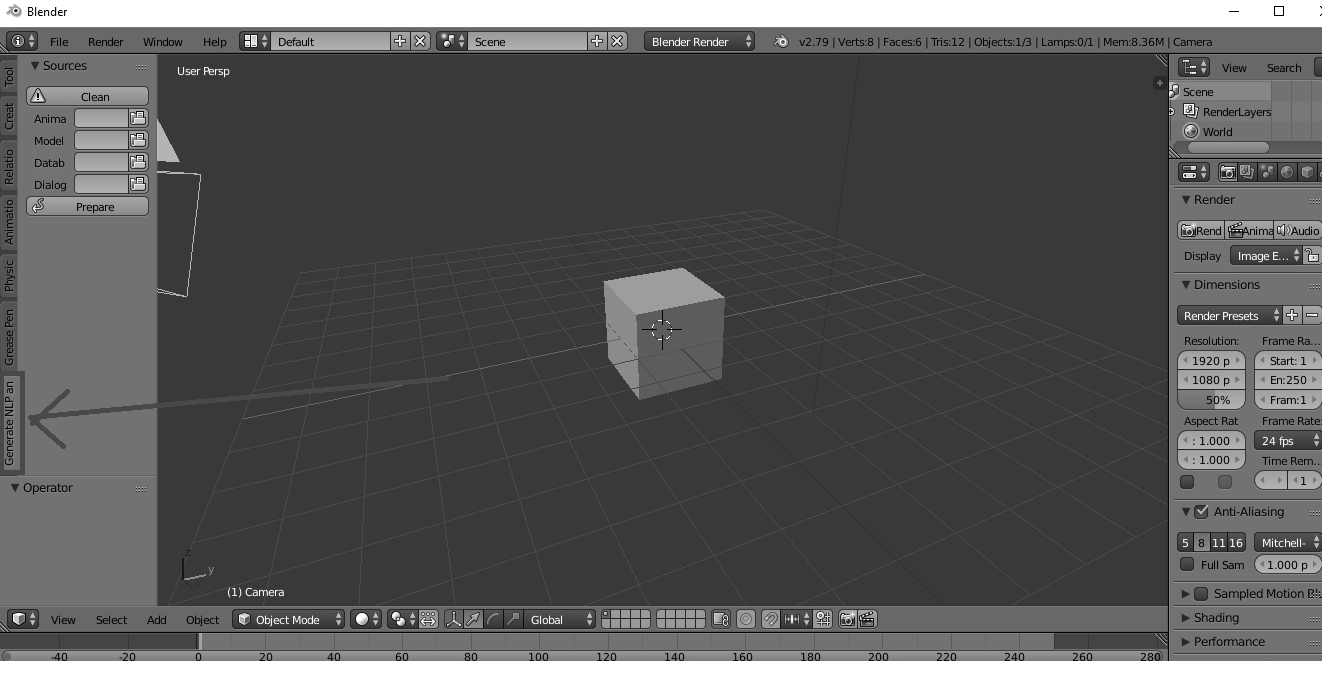
\includegraphics[width = 30em]{img/appendix/installedaddon.png}}}
	\caption{The generator addon menu}\label{fig:installedaddon}
\end{figure}

\section{Generating animations}
\noindent Now that all the requirements are met, the animation can be generated. There are two main steps to generating. Firstly, use the analyzer module to create a JSON file instructions for the generator. Secondly, use the generator to assemble the animation.

\subsubsection{Analyze script \label{sec:analyze-script}}
\noindent The input script must resemble the script in figure ~\ref{inputscript2}

\begin{figure}[!ht]
	\centerline{\fbox{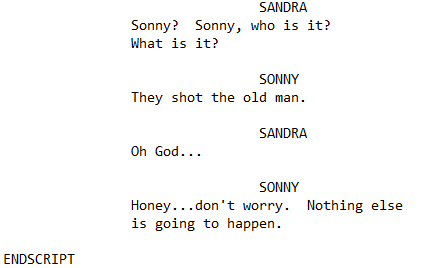
\includegraphics[width = 30em]{img/script.png}}}
	\caption{An example of system's input}\label{fig:inputscript2}
\end{figure}

\noindent The characters must be specified after 5 tabs. The dialogue text is specified after 3 tabs. The file must end with an `ENDSCRIPT` with no indentation. For reference please refer to either:
\begin{itemize}
	\item Example script files in folder `movies`
	\item Movie scripts hosted on \url{www.imsdb.com}
\end{itemize}

\noindent The script now can be process using the following command:

\indent `python analyzer/script\_analyze.py path\_to\_dialogue\_script db/animation.db`

\noindent The program will output a file called `scene.json`. This file is used to generate the animation.

\subsubsection{Generate Animation}
\noindent If you did not follow section ~\ref{sec:installaddon}, please follow these steps:
\begin{itemize}
	\item Open the file `rendered.blend` with Blender
	\item Click `Run Script` on the bottom of the scripting view (figure ~\ref{fig:withoutaddon})
	\item The tab called `Generate NLP anim` should appear on the right hand side menu of the 3D view
	\item Click on the `Generate NLP anim` tab
\end{itemize}

\begin{figure}[!ht]
	\centerline{\fbox{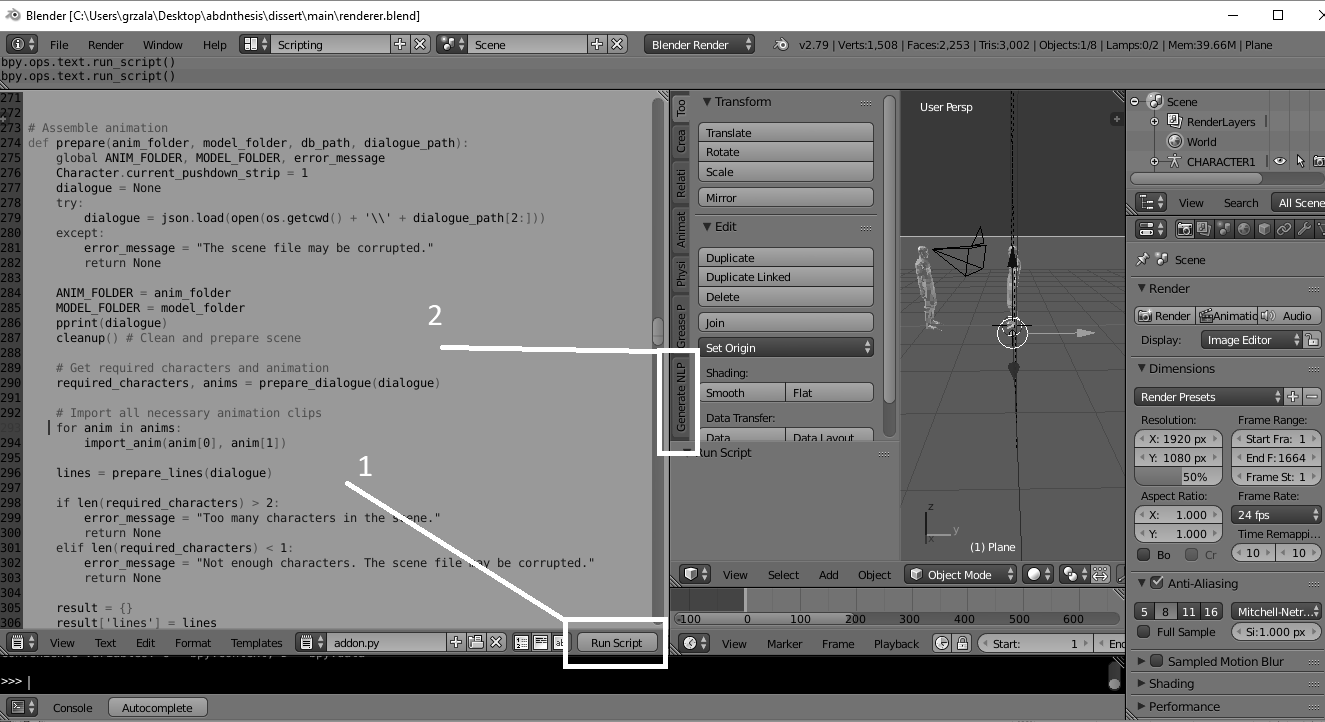
\includegraphics[width = 30em]{img/appendix/withoutaddon.png}}}
	\caption{Running the generator without installing it as an add-on}\label{fig:withoutaddon}
\end{figure}

Please follow these steps only if you installed the generator as an add-on:
\begin{itemize}
	\item Open Blender
	\item Press `File > Save` and save the file in a preferred location
	\item \textbf{Important:} close Blender and reopen the saved file
	\item Open `Generate NLP anim` tab
\end{itemize}

\noindent After finishing the above instructions, do the following to finalize the animation:
\begin{itemize}
	\item Press `Clean` at the top of the menu
	\item Choose the directory `mocap` for `Animations Directory`
	\item Choose the directory `models` for `Models Directory`
	\item Choose the file `db/animation.db` for `Database`
	\item For `Dialogue` choose the `scene.json` file you created when following the section ~\ref{sec:analyze-script}
	\item press `Prepare` 
\chapter{Maintenance Manual \label{chap:maintenance}}

\section{Installation and requirements}
For information on installation and dependencies please refer to sections ~\ref{sec:requirements} and ~\ref{sec:installaddon}.

\section{Space and Memory requirements}
The project needs enough memory to install Blender and Python as well as another 100MB to fit all the animation data. Please keep in mind that rendering the animations drastically increases the memory needed as one short clip may take up to 50MB. The project comes with a few example rendered videos which take another 150MB of memory

\section{Temporary Files}
When using the EMBD importer the program will store the downloaded EMBD BVH files in the `EMBD importer/tmp' directory. These files can take a considerable amount of space and can be deleted at the convenience of a user.

\section{Files and Directories}
The files and directories are described in tables ~\ref{tab:analyzerdirectory}, ~\ref{tab:dbdirectory}, ~\ref{tab:embd-importerdirectory}, ~\ref{tab:generatordirectory} and ~\ref{tab:maindirectory}.

\begin{table}[H]
	\centering
	\small
	
	\begin{tabular}{ |p{8.5em}|p{30.1em}| }
		\hline
		\multicolumn{2}{|c|}{\textbf{Main project directory}} \\
		\hline
		\thead{Item} & \thead{Description} \\
		\hline
		analyzer/ & The directory that contains the first and second module source code (emotion analysis and matcher) \\
		\hline
		db/ & The directory that contains the sqlite database file which holds information on the animations and models \\
		\hline
		EMBD importer/ & The directory that contains the EMBD importer tool \\
		\hline
		generator/ & The directory that contains the Blender add-on \\
		\hline
		mocap/ & The directory that contains the .fbx animations \\
		\hline
		models/ & The directory that contains the .fbx character models \\
		\hline
		movies/ & The directory that contains sample dialogue scripts \\
		\hline
		showcases/ & The directory that contains sample rendered scenes \\
		\hline
		rendered.blend & Blender project prepared for use with the system \\
		\hline
	\end{tabular}
	
	\caption{Contents of the main directory}
	\label{tab:maindirectory}
\end{table}

\begin{table}[H]
	\centering
	\small
	
	\begin{tabular}{ |p{8.5em}|p{30.1em}| }
		\hline
		\multicolumn{2}{|c|}{\textbf{`analyzer' directory}} \\
		\hline
		\thead{Item} & \thead{Description} \\
		\hline
		db.py & The source code of the matcher module \\
		\hline
		generate\_showcase.py & The source code of the showcase generator (more information in sections ~\ref{sec:showcasegenerator} and ~\ref{sec:showcasegeneratormanual}) \\
		\hline
		parse.py & Script used to parse the dialogue script \\
		\hline
		script\_analyze.py & The main file of the analyzer program. It handles the resource pipeline. \\
		\hline
		tone.py & The script that uses the IBM Watson API to perform emotion analysis \\
		\hline
	\end{tabular}
	
	\caption{Contents of the `analyzer' directory}
	\label{tab:analyzerdirectory}
\end{table}

\begin{table}[H]
	\centering
	\small
	
	\begin{tabular}{ |p{8.5em}|p{30.1em}| }
		\hline
		\multicolumn{2}{|c|}{`db' directory} \\
		\hline
		\thead{Item} & \thead{Description} \\
		\hline
		animation.db & The sqlite file that holds the information on the animations and character models \\
		\hline
	\end{tabular}
	
	\caption{Contents of the `db' directory}
	\label{tab:dbdirectory}
\end{table}

\begin{table}[H]
	\centering
	\small
	
	\begin{tabular}{ |p{8.5em}|p{30.1em}| }
		\hline
		\multicolumn{2}{|c|}{\textbf{`EMBD importer' directory}} \\
		\hline
		\thead{Item} & \thead{Description} \\
		\hline
		imported/ & The directory that holds the imported animations \\
		\hline
		tmp/ & The directory that caches downloaded EMBD animations \\
		\hline
		armature.fbx & Character armature used for reference during importing. This armature is used for all the animations in the project \\
		\hline
		importer.blend & Blender project prepared to handle importing animations from EMBD \\
		\hline
		script.py & Source code of the importer. This script is meant to be run from inside of Blender \\
		\hline
	\end{tabular}
	
	\caption{Contents of the `EMBD importer' directory}
	\label{tab:embd-importerdirectory}
\end{table}

\begin{table}[H]
	\centering
	\small
	
	\begin{tabular}{ |p{8.5em}|p{30.1em}| }
		\hline
		\multicolumn{2}{|c|}{\textbf{`generator' directory}} \\
		\hline
		\thead{Item} & \thead{Description} \\
		\hline
		addon.py & The source code of the generator module \\
		\hline
	\end{tabular}
	
	\caption{Contents of the `generator' directory}
	\label{tab:generatordirectory}
\end{table}


\section{Known Issues}
\noindent Please make sure that the dialogue script is correctly formatted before running the emotion analysis. Wrong indentation levels may cause unpredictable results.

\noindent The generator module will provide you with an error message if the input (scene.json) is malformed. However if the file parses correctly but it's data is corrupted it may lead to unpredictable results. This situation will never take place is the scene.json file was generated by the script\_analyze.py program.



\chapter{Other \label{chap:otherappendices}}

\section{The questionnaire \label{sec:appquestionnaire}}

\begin{figure}[h]
	\makebox[\textwidth][c]{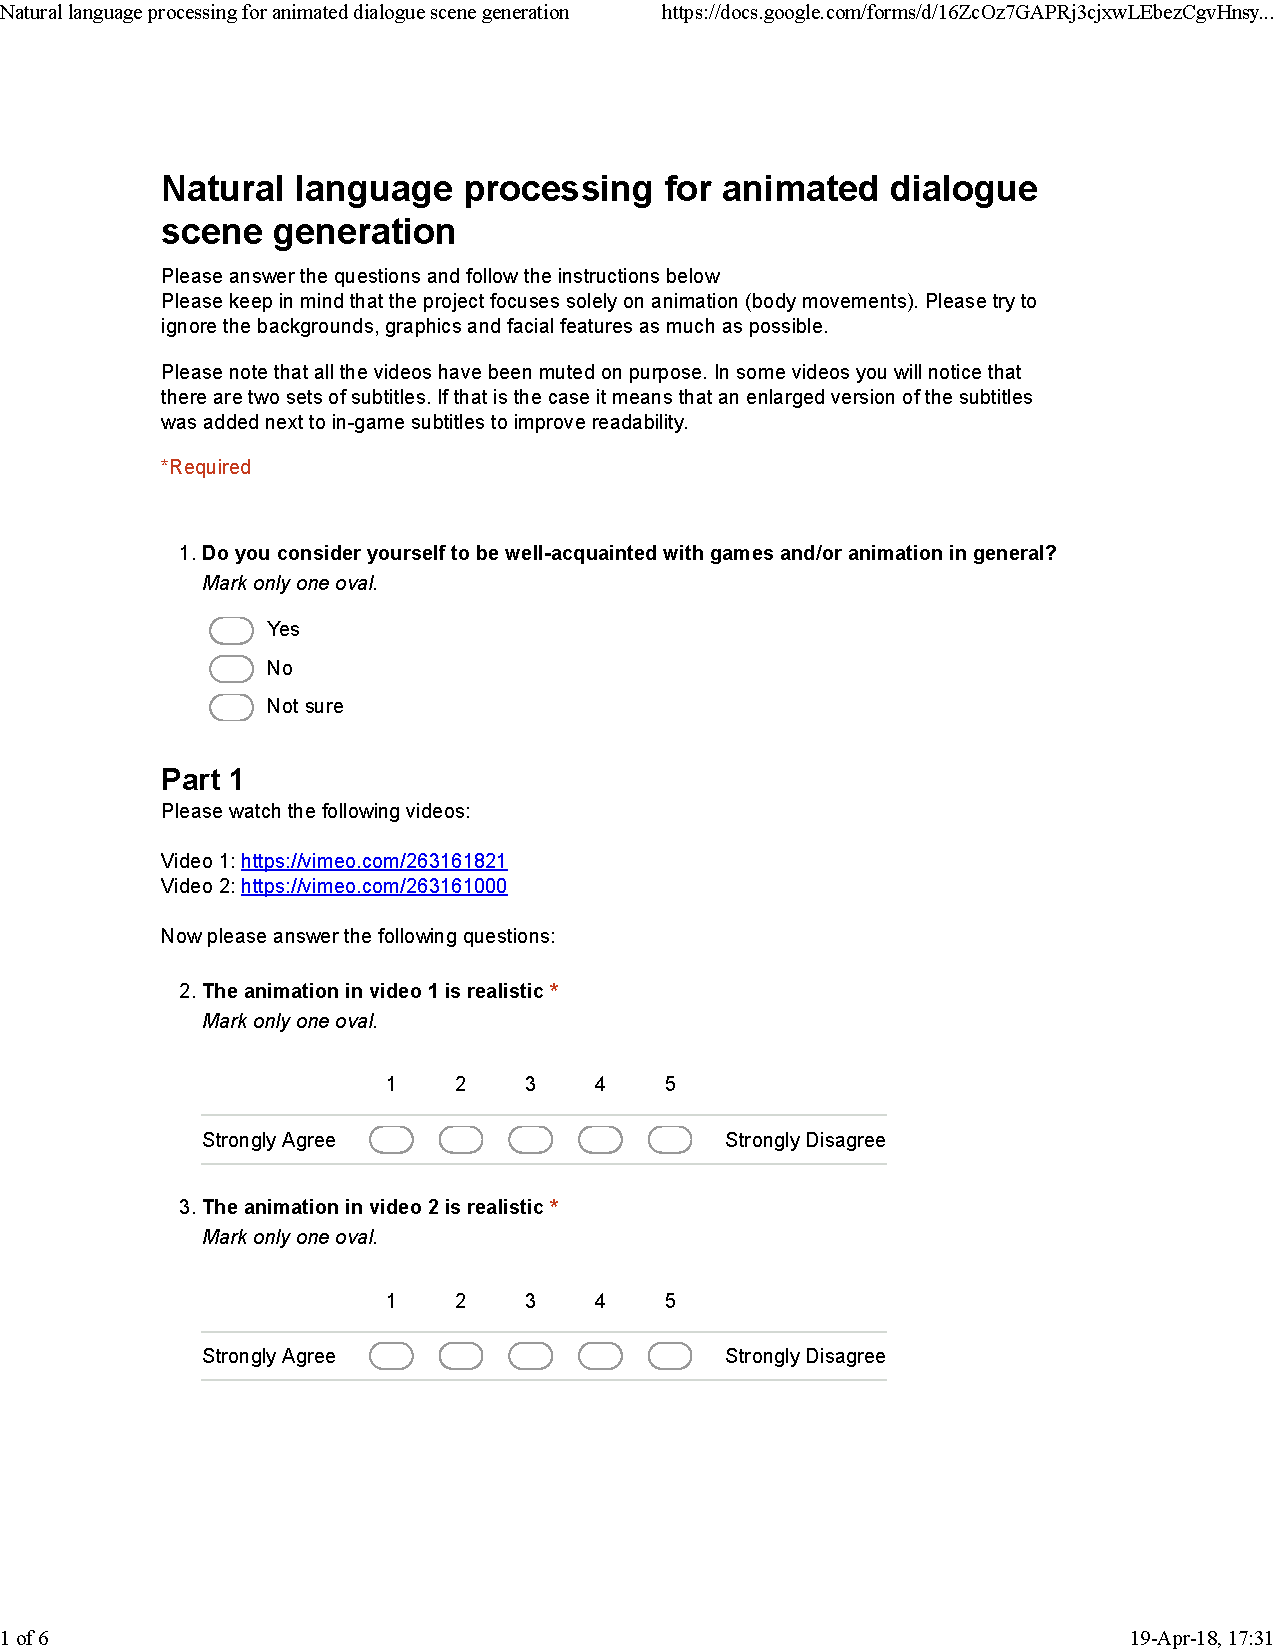
\includegraphics[page=1,width=1.2\textwidth]{img/appendix/questionnaire.pdf}}
	\caption{The questionnaire - page 1}
\end{figure}

\begin{figure}[h]
	\makebox[\textwidth][c]{\includegraphics[page=2,width=1.2\textwidth]{img/appendix/questionnaire.pdf}}
	\caption{The questionnaire - page 2}
\end{figure}

\begin{figure}[h]
	\makebox[\textwidth][c]{\includegraphics[page=3,width=1.2\textwidth]{img/appendix/questionnaire.pdf}}
	\caption{The questionnaire - page 3}
\end{figure}

\begin{figure}[h]
	\makebox[\textwidth][c]{\includegraphics[page=4,width=1.2\textwidth]{img/appendix/questionnaire.pdf}}
	\caption{The questionnaire - page 4}
\end{figure}

\begin{figure}[h]
	\makebox[\textwidth][c]{\includegraphics[page=5,width=1.2\textwidth]{img/appendix/questionnaire.pdf}}
	\caption{The questionnaire - page 5}
\end{figure}

\begin{figure}[h]
\makebox[\textwidth][c]{\includegraphics[page=6,width=1.2\textwidth]{img/appendix/questionnaire.pdf}}
\caption{The questionnaire - page 6}
\end{figure}

\end{document}
